\chapter{Introduction} \label{ch:intro}
The discovery of new pharmaceuticals traditionally follows the design-make-test paradigm, where molecules are repeatedly proposed, synthesized, and assayed. Drug candidates are designed based on some hypothesis relating chemical structure to drug activity, which gets updated in light of new activity results. This cycle repeats as the molecular search space narrows down until a candidate molecule satisfies the necessary activity/selectivity/toxicity criteria.

\begin{figure}[!h] % !h ~ force here, t ~ top, b ~ bottom, p ~ separate page
    \centering
    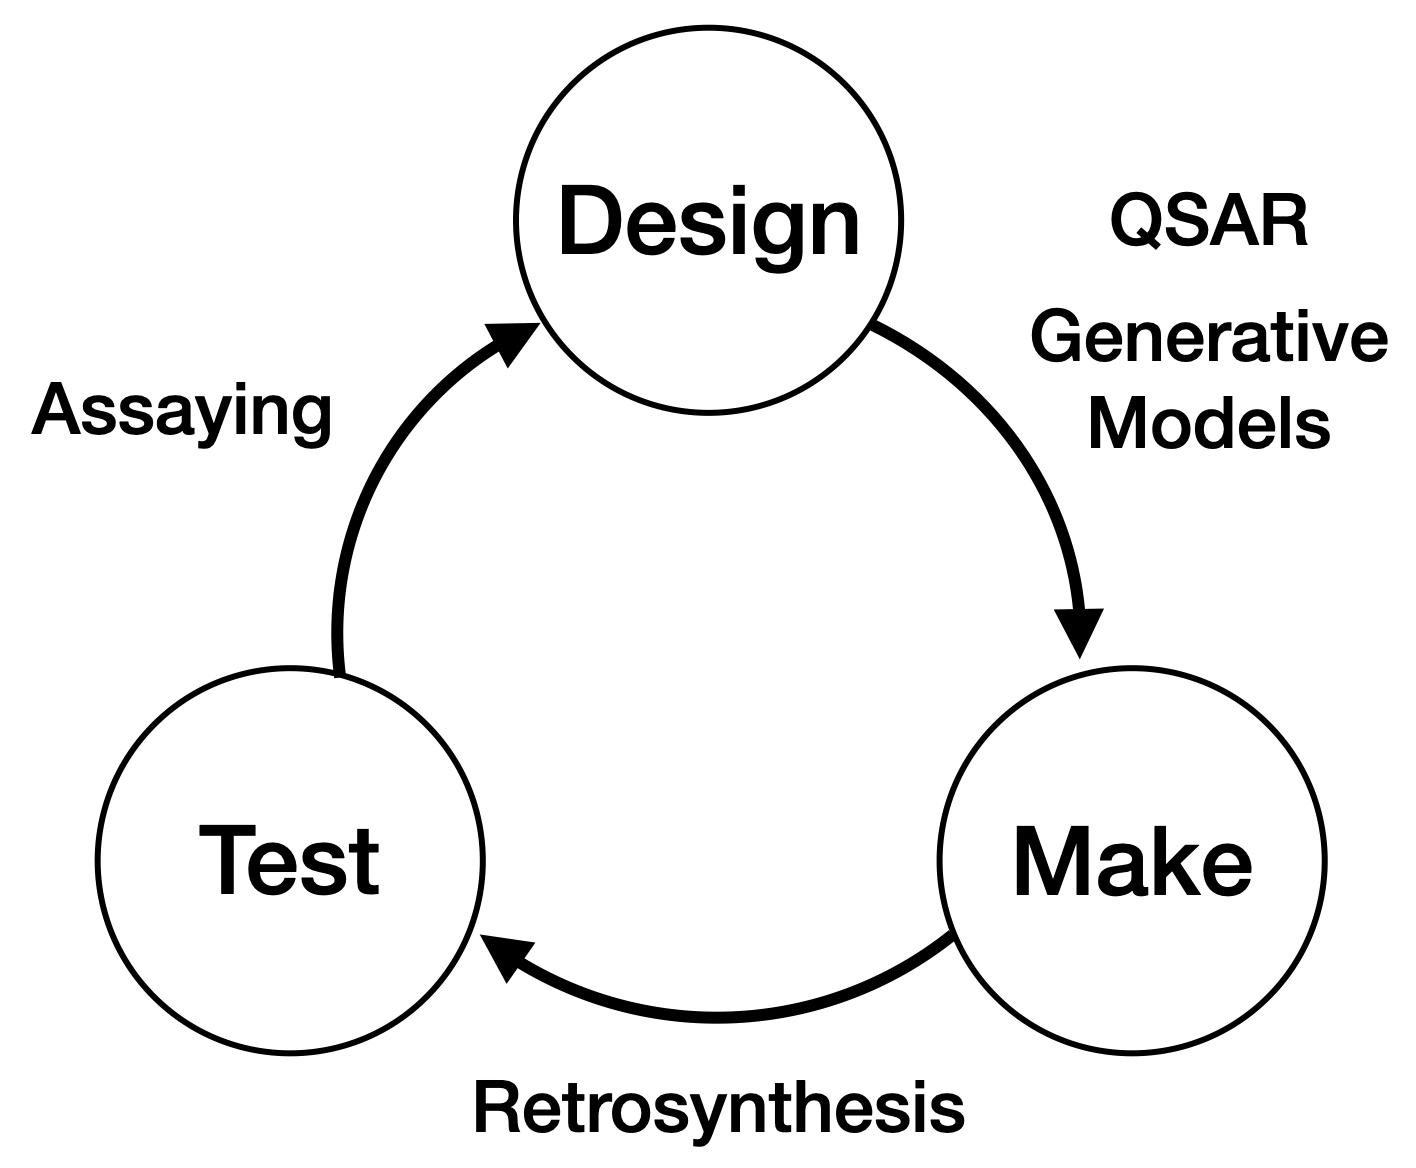
\includegraphics[width=0.5\textwidth]{Chapters/Intro/Figs/design-make-test.png}
    \caption{\label{fig:cycle} An overview of the design-make-test cycle in drug discovery.}
\end{figure}

While computational methods have long been used in various stages of the cycle, there has been a recent surge in applying artificial intelligence to drug discovery following its success in various other fields, most notably computer vision and natural language processing. Since molecular assaying is largely an automated process the application focus has been on `design' and `make' \cite{Coley2019AutonomousProgress}, for example in modelling quantitative structure-activity relationships (QSAR), designing generative models for proposing drug candidates, and planning retrosynthesis routes (Fig~\ref{fig:cycle}). 

As the field of data-driven drug discovery matures beyond merely adapting the latest state-of-the-art machine learning (ML) methods, the present challenge is to tailor ML models specifically for the unique problems and situations faced in pharmaceutical chemistry. This report summarizes my efforts over the past year to play a part in this challenge with intuitions based on physical science. These consist of three separate tasks, one on `Make' and two on `Design':

\section*{Design}
The research presented in this thesis explore ways in which data-driven approaches based on machine learning can be leveraged in the design-make-test cycle of drug discovery. In each of the three steps of `design', `make', and `test' we encounter the same underlying challenge, of grappling with the practical difficulties of a drug discovery campaign where we must make full use of the limited data available.

In Chapter \ref{ch:fresco} we looked at how to leverage fragment-protein structures from a crystallographic fragment screen to hit discovery in the absence of any bioactivity data. Using an unsupervised learning approach, we learn the geometric distribution of pharmacophores from the fragment-protein complexes, and use these to screen potential molecules for bioactivity. We showed that this approach outperforms docking on distinguishing active compounds from inactive ones on retrospective data. Further, we prospectively found novel hits for SARS-CoV-2 Mpro and the Mac1 domain of SARS-CoV-2 non-structural protein 3 by virtually screening a library of 1B molecules.

Chapter \ref{ch:ranking} takes us to the early stages of hit-to-lead molecular optimisation where bioactivity data is limited, noisy, and dominated by inactive molecules. We overcame this challenge with a learning-to-rank framework via an ML model that predicts whether a compound is more or less active than another. This approach allowed us to make use of inactive data and threshold the bioactivity differences above measurement noise, and validation on retrospective data for SARS-CoV-2 Mpro showed that we can outperform docking on ranking ligands. Combining this model with AI-based synthesis tools, we prospectively screened a library of 8.8M molecules to arrive at a potent compound with a novel scaffold.

\section*{Make}
While AI-based synthesis tools have already shown demonstrable success in accelerating the synthesis of new molecules, they are still prone to failure and suffer from a lack of transparency in their decision making due to their black-box nature. To address this, in Chapter \ref{ch:transformer} we showcased a workflow for quantitatively interpreting a state-of-the-art deep learning model for reaction prediction. By analysing chemically selective reactions, we showed examples of correct reasoning by the model, explain counterintuitive predictions, and identify Clever Hans predictions where the correct answer is reached for the wrong reason due to dataset bias.

\section*{Test}
In Chapter \ref{ch:testing} we explored how to accelerate testing procedures by applying machine learning on bioactivity data from nanomolar-scale high-thoughput chemistry. While this experimental technique greatly increases the number of molecules that can be tested, there is additional noise resulting from having to assay crude reaction mixtures instead of pure samples. Nevertheless, we showed that machine learning models trained on this data is able to cut through this noise and identify a false negative assay measurement, as well as prospectively screen a library of ~62K molecules to discover new SARS-CoV-2 Mpro inhibitors just as potent as those from the original assay.

% The process of drug discovery can be summarised by the design-make-test cycle, where molecules are repeatedly proposed, synthesized, and assayed until a suitable drug candidate is found. Machine learning (ML) approaches are increasingly used to accelerate and automate all parts of this process \cite{Coley2019AutonomousOutlook, Coley2019AutonomousProgress}. The focus of the current thesis is the ``make'' part of the cycle. This is of interest because the synthesis of putative drug molecules is the most time consuming and labour intensive part of the cycle. As Blakemore et. al. \cite{Blakemore2018OrganicDiscovery} puts it ``Organic synthesis is certainly not a solved problem''. The most crucial part of the synthesis is route planning, traditionally done by expert chemists who are following the so-called disconnection approach \cite{Warren2011OrganicApproach} which is the classical framework for designing synthesis plans. Chemists usually rely on their own experience and domain knowledge, as well as databases of reactions like Reaxys \cite{ElsevierReaxysDatabase}. Nowadays, increasingly and with some success Computer Assisted Synthesis Planning tools are being used to help the chemists in designing better reaction plans \cite{Coley2018}. These tools have several advantages compared to humans: Firstly, they can quickly evaluate a very large number of possible disconnections via efficient algorithms such as Monte Carlo Tree Search \cite{Segler2018PlanningAIb}. Furthermore, by having access to exhaustive libraries of commercially available building blocks the models can disconnect into large and complex starting materials that can be readily purchased. This can reduce the number of steps and hence the risk of failure substantially. \par
% Once a feasible disconnection is found it is important to validate each step of the plan. Forward chemical reaction prediction is concerned with predicting the (major) product of an organic reaction given the reactants, reagents and preferably the conditions like solvent, temperature, concentrations etc. By having the ability to predict the product of reactions with reliable uncertainties it is possible to design clever synthesis plans where the reactions with higher uncertainty are put first. This way if a synthesis protocol fails it does so fast and cheap instead of in the later stages of the route where substantial time and cost would go to waste.\par
% The most successful approaches to forward reaction prediction all rely on machine learning \cite{Coley2018, Schwaller2019MolecularPrediction}. These models are trained on reaction data that is extracted from patents and publications. In these documents usually the metadata about reactions like the temperature, concentrations and solvents are found in the synthesis protocol section making it very challenging to extract this information in an automated manner. That is why these models are usually trained only on the reactants and reagents with all of the context information missing. There have been attempts at predicting the yield of the reactions as well, but they concluded that it was only possible to predict them for high throughput experiments \cite{Schwaller2020PredictionLearning} .This is largely because the yield (and sometimes even the major product) is highly dependent on the conditions making the reaction prediction task from only reactants and reagents to products ill-defined. In spite of this there are reported models achieving remarkably high near 90\% Top-1 prediction accuracy on these datasets. Therefore it is of utmost importance to validate these models to see if they are able to generalize and predict the outcome of reactions reliably or if they are learning hidden biases in the datasets which results in the seemingly strong performance. \par
% One way to accomplish this is with ML interpretability methods. These methods are being used increasingly in the machine learning community as a tool for evaluating model robustness \cite{Alvarez-Melis2018OnMethods}. This is especially the case in scientific applications where there is usually a large amount of prior knowledge about the systems from classical physics or chemistry. Interpretability methods can help uncover the reasoning of the models predictions in simple well understood cases where the physical or chemical cause for certain outcomes is well established. This is certainly the case for chemical reaction prediction where our understanding of mechanisms and selectivities serve as good guides for the observed reactivities. If a failure in the model's understanding is uncovered this way, a number of adversarial examples (experiments) can be designed which can than be fed back into the model as new training data. This is similar to an active learning cycle that is driven by the interpretability and human understanding of the underlying chemistry. \par
% A further factor necessitating interpretability in scientific machine learning is the nature of scientific data. For example in the case of chemical reaction prediction there are a number of known or hidden biases in the commonly used datasets. One of the well-known biases is the lack of negative results, meaning that every training reaction has a good outcome. This is in contrast to reality when often if a few chemicals are mixed there is no reaction, or no well defined reaction happening. This is something the models are not able to learn from only seeing positive data.\par
% Last but not least, interpretability methods can be used as a tool for imputing missing metadata. In the case of reaction prediction if a model can not only predict the outcome of a reaction but it can also return a number of similar training reactions with their sources (patent ID or DOI) than these can be used by the chemist to infer what the ideal conditions (solvents, temperature etc.) are for the predicted product to be realized in the lab. We believe that this novel use of interpretability can be of great use in the reaction prediction community. \par
% In Chapter~\ref{chap:backgroun} an introduction to forward chemical reaction prediction is given. The most important approaches are reviewed, including \textit{ab initio} quantum mechanics based, rule based and template free machine learning methods. The Molecular Transformer \cite{Schwaller2019MolecularPrediction} is presented in detail. This is the current state-of-the-art reaction prediction model in terms of Top-1 accuracy on a standard benchmark dataset, and the interpretation of this model is the focus of the current work. \par
% In Chapter~\ref{chap:methods} a short review of interpretable machine learning is given. The term ``interpretability'' in the context of reaction prediction and this work is defined, and our methods for interpretation are presented in detail. This includes the Integrated Gradients method \cite{Sundararajan2017AxiomaticNetworks} which has been used for interpreting chemistry models before. We build on the work of McCloskey et. al. \cite{McCloskey2019UsingChemistry} who used IGs to understand binding prediction models on artificial datasets. We extend the method to Transformer architectures, and use it in the context of reaction predictions on real experimental data. We also present a novel method for attributing the predictions of neural network models to training data points. This is a new way of thinking about interpretation that has not been used before and that can be of great use in the reaction prediction domain. \par
